\documentclass[tikz,border=8pt]{standalone}
\usepackage[T1]{fontenc}
\usepackage{lmodern}
\usetikzlibrary{arrows.meta,fit,positioning}
\definecolor{controlblue}{HTML}{0072B2}
\definecolor{dataorange}{HTML}{B85C00}
\tikzset{
  component/.style={draw=black!55,fill=black!3,rounded corners=2pt,
    minimum width=31mm,minimum height=12mm,align=center,font=\sffamily\small},
  edge/.style={-{Latex[length=2.5mm]},line width=1pt},
  control/.style={edge,draw=controlblue},
  data/.style={edge,draw=dataorange,dashed},
  relation/.style={draw=black!55,line width=.8pt},
  label/.style={font=\sffamily\scriptsize,align=center},
  boundary/.style={draw=black!40,rounded corners=4pt,inner sep=8mm}
}
% The agent replaces these labels and Evidence IDs with recovered records.
% The agent changes sample nodes and edges to match actual evidence.
\newcommand{\SystemLabel}{Original application}
\newcommand{\EntryLabel}{C-001\\Entry component}
\newcommand{\CoreLabel}{C-002\\Processing component}
\newcommand{\ResultLabel}{C-003\\Output component}
\newcommand{\CallEvidence}{EDGE-001 / E-001 / unknown}
\newcommand{\DataEvidence}{EDGE-002 / E-002 / unknown}
\newcommand{\ActionLabel}{Invoke interface}
\newcommand{\PayloadLabel}{Transfer result}
\begin{document}
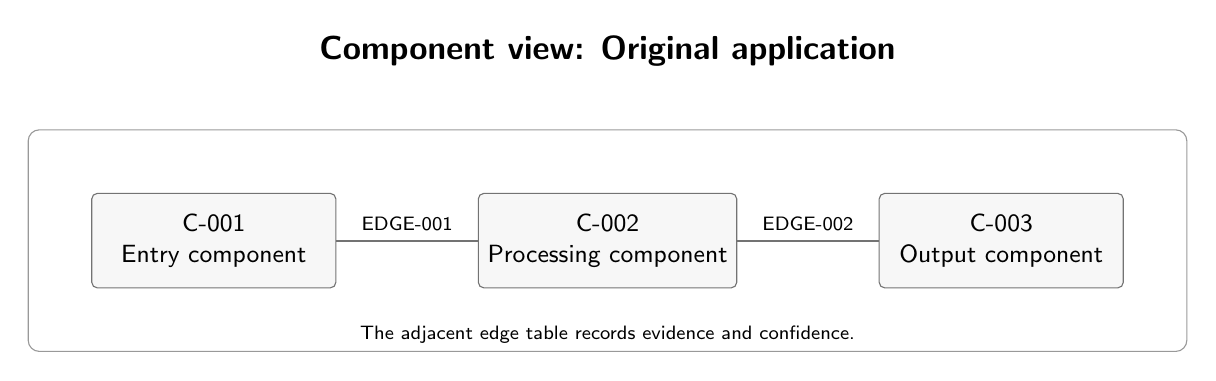
\begin{tikzpicture}
  \node[font=\sffamily\bfseries\large] at (5,2.4) {Component view: \SystemLabel};
  \node[component] (entry) at (0,0) {\EntryLabel};
  \node[component] (core) at (5,0) {\CoreLabel};
  \node[component] (result) at (10,0) {\ResultLabel};
  \node[boundary,fit=(entry)(core)(result)] {};
  \draw[relation] (entry.east) -- node[label,above] {EDGE-001} (core.west);
  \draw[relation] (core.east) -- node[label,above] {EDGE-002} (result.west);
  \node[label] at (5,-1.2) {The adjacent edge table records evidence and confidence.};
\end{tikzpicture}
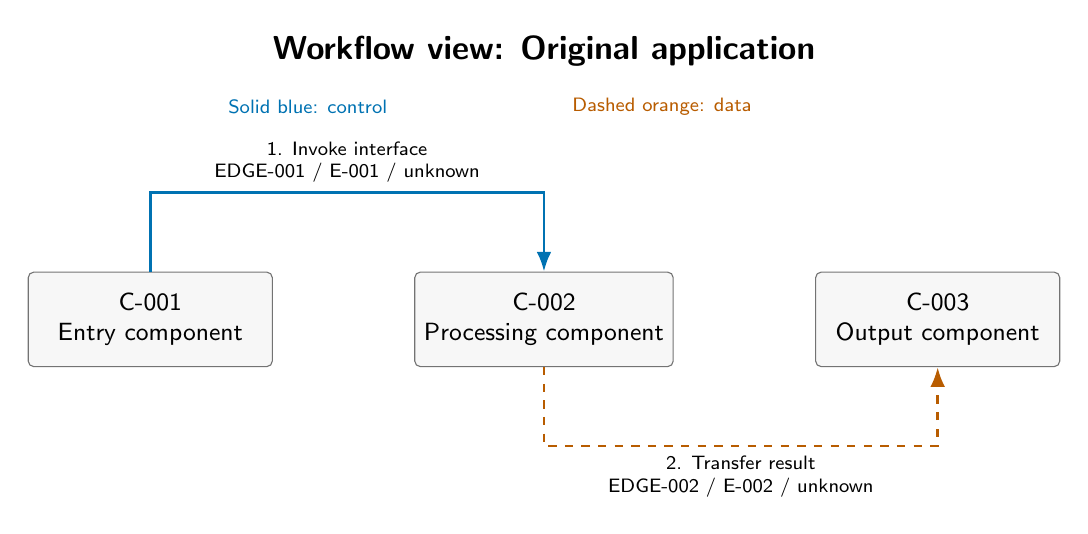
\begin{tikzpicture}
  \node[font=\sffamily\bfseries\large] at (5,3.4) {Workflow view: \SystemLabel};
  \node[component] (entry) at (0,0) {\EntryLabel};
  \node[component] (core) at (5,0) {\CoreLabel};
  \node[component] (result) at (10,0) {\ResultLabel};
  \draw[control] (entry.north) -- ++(0,1) -| node[label,above,pos=.25]
    {1. \ActionLabel\\\CallEvidence} (core.north);
  \draw[data] (core.south) -- ++(0,-1) -| node[label,below,pos=.25]
    {2. \PayloadLabel\\\DataEvidence} (result.south);
  \node[label,text=controlblue] at (2,2.7) {Solid blue: control};
  \node[label,text=dataorange] at (6.5,2.7) {Dashed orange: data};
\end{tikzpicture}
\end{document}
